\section{Online Job Scheduling}
In this section,  we explore the role of calibration in a model for \textit{scheduling with predictions} first proposed by \citet{Cho22:Scheduling} to direct 
human review of ML-flagged abnormalities in diagnostic radiology. Omitted proofs from this section can be found in \cref{appendix: scheduling-proofs}. 
\subsection{Setup}
\paragraph{Problem.} There is a single machine (lab tech) that needs to process $n$ jobs (diagnostic images), each requiring one unit of processing time. Job $i$ has some unknown priority $y_i\in\{0,1\}$ that is independently high $(y_i=1)$ with probability $\rho$ and low $(y_i=0)$ with probability $1-\rho$. Although job priorities are unknown a priori, the priority $y_i$ is revealed after completing some fixed fraction $\theta \in (0,1)$ of job $i$. Upon learning $y_i$, a scheduling algorithm can choose to complete job $i$, or switch to a new job and ``store" job $i$ for completion at a later time. The goal is to schedule the $n$ jobs in a way that minimizes the weighted sum of completion times $\sum_{i=1}^n C_i \cdot \omega_{y_i}$
where $C_i$ is the completion time of job $i$, and $\omega_1 >\omega_0 >0$ are costs associated with delaying a job of each priority for one unit of time. In hindsight, it is optimal to schedule jobs in decreasing order of priority.

\paragraph{ML predictions.}
 Based on the assumption that the $n$ jobs to be scheduled are iid, let $\cX = \cX_0^n$ be a set of job features, $\cI = \{0,1\}^n$ be the set of possible priorities, and $\cD = \cD_0^n$ be an unknown joint distribution over feature/priority pairs. The prediction task for this problem involves training a predictor $f$ whose target is the true priority of each job $T(\vec{y}) = \vec{y}$. This amounts to training a 1-dimensional predictor $f: \mathcal{X}_0 \to \cZ$ that acts on the $n$ jobs independently:
 $f(\vec{X}) := (f(\vec{X}_1), \dots, f(\vec{X}_n)).$
 
\paragraph{Prediction-aided scheduling.}
\citet{Cho22:Scheduling} introduce a threshold-based scheduling rule informed by probabilities $p_i$ that job $i$ is high priority based on identifying features (\cref{alg: beta-threshold}). Their algorithm switches between two extremes---a \textit{preemptive} policy that starts a new job whenever the current job is revealed to be low priority, and a \textit{non-preemptive} policy that completes any job once it is begun---based on the threshold parameter \[\beta := \frac{\theta}{1 - \theta} \cdot \frac{\omega_1}{\omega_1 - \omega_0}.\]
In detail, jobs are opened in decreasing order of $p_i$. Jobs with $p_i > \beta$ are processed preemptively, and the remaining jobs are processed non-preemptively.

 \begin{algorithm}[b]
   \caption{$\beta$-threshold rule}
    \label{alg: beta-threshold}
\begin{algorithmic}
   \STATE {\bfseries input: }Probabilities $\{p_i\}_{i=1}^n$ that each job is high-priority
   \STATE Define $n_1 = |\{i: p_i > \beta\}|$ \\
   \STATE Order probabilities $p_{(1)} \geq \dots \geq p_{(n)}$\\
   \STATE Run jobs $j_{(1)}, \dots, j_{(n_1)}$ preemptively, in order
   \STATE Complete remaining jobs non-preemptively, in order
\end{algorithmic}
\end{algorithm}

A prediction-aided algorithm $\cA$ for job scheduling determines the probabilities $p_i$ from ML advice. \citet{Cho22:Scheduling} assume access to a binary predictor $f_b: \cX_0 \to \{0,1\}$ of job priority and study the case where $p_i = \Pr[\vec{Y}_i=1 \mid f_b(\vec{X}_i)]$. These probabilities can be computed using Bayes' rule, and because $f_b$ is binary, this procedure effectively assigns each job one of two probabilities. Although not explicitly discussed by \citet{Cho22:Scheduling}, this amounts to a basic form of post-hoc calibration. In contrast, our results extend to arbitrary calibrated predictors $f: \cX_0 \to [0,1]$---a more general framework that calls for new mathematical techniques---allowing us to significantly improve upon their results. In this setting, $\cA$ takes the predictions $f(\vec{X})=\vec{v}$ as input and executes \cref{alg: beta-threshold} with probabilities $p_i=\vec{v}_i$.

To quantify the optimality gap of $\cA$, \citet{Cho22:Scheduling} note that compared to \OPT, \cref{alg: beta-threshold} incurs (1) a cost of $\theta \omega_1$ for each \textit{inversion}, or pair of jobs whose true priorities $y_i$ are out of order, and (2) a cost of $\theta \omega_0$ for each pair of low priority jobs encountered when acting preemptively. When acting non-preemptively, \cref{alg: beta-threshold} incurs (3) a cost of $\omega_1 - \omega_0$ for each inversion. Thus, for fixed predictions $f(\vec{X}) = \vec{v}$ and true job priorities $\vec{y}$,
 \begin{equation}\label{eq:scheduling_CR}
    \ALG(\cA, \vec{v}, \vec{y}) - \OPT(\vec{y}) = \theta\omega_1 L(\vec{v}, \vec{y}) + \theta\omega_0  M(\vec{v}, \vec{y}) + (\omega_1 - \omega_0)  N(\vec{v}, \vec{y}),
 \end{equation}
 where $L(\vec{v}, \vec{y}), M(\vec{v}, \vec{y}),$ and $N(\vec{v}, \vec{y})$ count occurrences of (1), (2), and (3), respectively (see \cref{table: data-description} for details).
\begin{table*}[!tb] 
\centering
\small
    \caption{Quantities of interest in prediction-aided scheduling for fixed predictions $f(\vec{X})=\vec{v}$ and job priorities $\vec{y}$.}
    \label{table: data-description}
\begin{tabular}{lp{5.5cm}l}
\toprule
\textbf{Quantity}  & \textbf{Description} &\textbf{Relevant setting} \\
\midrule
$n_1 = |\{i: \vec{v}_i > \beta\}|$ & Number of jobs likely to be high priority. & ---\\
$L(\vec{v}, \vec{y}) = \displaystyle\sum_{i=1}^{n_1} \sum_{j = i+1}^{n_1} \mathbbm{1}_{\{\vec{y}_{(i)} = 0 \land \vec{y}_{(j)} = 1\}}$ & Number of inversions among jobs likely to be high priority. & Preemptive \\
$M(\vec{v}, \vec{y}) = \displaystyle\sum_{i=1}^{n_1} \sum_{j = i+1}^{n_1} \mathbbm{1}_{\{\vec{y}_{(i)} = 0 \land \vec{y}_{(j)} = 0\}}$ & Number of low-priority job pairs among jobs likely to be high priority. & Preemptive\\
$N(\vec{v}, \vec{y}) = \displaystyle\sum_{i=1}^{n} \sum_{j = i+1}^{n}  \mathbbm{1}_{\{\vec{y}_{(i)} = 0 \land \vec{y}_{(j)} = 1\}} - L(\vec{v}, \vec{y})$ & Number of inversions among job pairs where at least one is likely to be low priority. & Non-preemptive\\

\bottomrule
\end{tabular}
\end{table*}

\subsection{Scheduling with calibrated predictions}
\paragraph{Calibration and job sequencing.} To build intuition for why finer-grained calibrated predictors sequence jobs more accurately, we begin by observing that \cref{alg: beta-threshold} orders jobs with the same probability $p_i$ randomly. Given a calibrated predictor $f$, consider the coarse calibrated predictor
\[
    f'(x) = \begin{cases}\E[f(X) \mid f(X) > \beta] & \text{if $f(x) > \beta$} \\
    \E[f(X) \mid f(X) \leq \beta] &\text{if $f(x) \leq \beta$}\end{cases}
\]

obtained by averaging the predictions of $f$ above and below the threshold $\beta$. Whereas $|R(f)|$ may be large, $f'$ is only capable of outputting $|R(f')|=2$ values. As a result, when ordering jobs with features $X_1, \dots, X_n$ according to predictions from $f'$, all jobs with $f(X) > \beta$ will be sequenced before jobs with $f(X) \leq \beta$, but the ordering of jobs within these bins will be random. In contrast, predictions from $f$ provide a more informative ordering of jobs (\cref{fig: job-seq}). Note, however, that $f = f'$ when $f$ has no variance in its predictions above or below the threshold $\beta$. We demonstrate in \cref{thm: schedule-improv} that this intuition holds in general --- improvements scale with the granularity of predictions.

\begin{figure}[htb]
    \centering
    \vskip 0.1in
   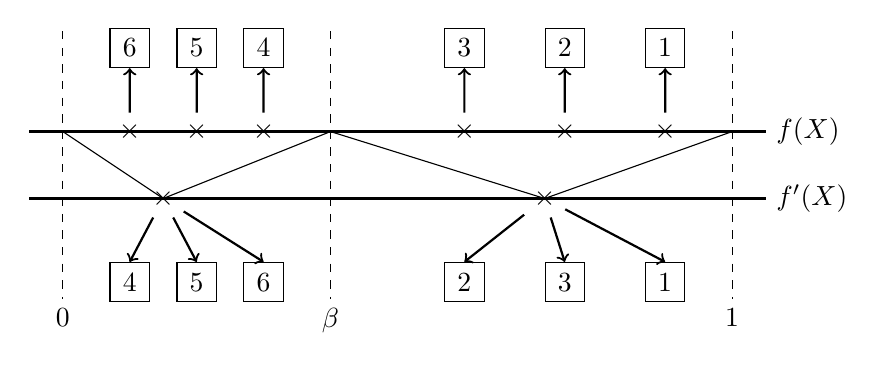
\begin{tikzpicture}[scale=0.85]

\draw[very thick] (-0.5,0.5) -- (10.5,0.5) node[right] {$f(X)$};
\draw[very thick] (-0.5,-0.5) -- (10.5,-0.5) node[right] {$f'(X)$};

\draw[dashed] (0,2) -- (0,-2) node[below] {$0$};
\draw[dashed] (4,2) -- (4,-2) node[below] {$\beta$};
\draw[dashed] (10,2) -- (10,-2) node[below] {$1$};
\draw[] (0, 0.5) -- (1.5, -0.5) {};
\draw[] (4, 0.5) -- (1.5, -0.5) {};
\draw[] (4, 0.5) -- (7.2, -0.5) {};
\draw[] (10, 0.5) -- (7.2, -0.5) {};

\node (x1) at (1, 0.5) {$\times$};
\node (x2) at (2, 0.5) {$\times$};
\node (x3) at (3, 0.5) {$\times$};
\node (x7) at (1.5, -0.5) {$\times$};

\node (x4) at (6, 0.5) {$\times$};
\node (x5) at (7.5, 0.5) {$\times$};
\node (x6) at (9, 0.5) {$\times$};
\node (x8) at (7.2, -0.5) {$\times$};

\node[draw, minimum width=0.5cm, minimum height=0.5cm] (box1) at (1, 1.75) {6};
\node[draw, minimum width=0.5cm, minimum height=0.5cm] (box2) at (2, 1.75) {5};
\node[draw, minimum width=0.5cm, minimum height=0.5cm] (box3) at (3, 1.75) {4};
\node[draw, minimum width=0.5cm, minimum height=0.5cm] (box4) at (6, 1.75) {3};
\node[draw, minimum width=0.5cm, minimum height=0.5cm] (box5) at (7.5, 1.75) {2};
\node[draw, minimum width=0.5cm, minimum height=0.5cm] (box6) at (9, 1.75) {1};

\node[draw, minimum width=0.5cm, minimum height=0.5cm] (box7) at (1, -1.75) {4};
\node[draw, minimum width=0.5cm, minimum height=0.5cm] (box8) at (2, -1.75) {5};
\node[draw, minimum width=0.5cm, minimum height=0.5cm] (box9) at (3, -1.75) {6};
\node[draw, minimum width=0.5cm, minimum height=0.5cm] (box10) at (6, -1.75) {2};
\node[draw, minimum width=0.5cm, minimum height=0.5cm] (box11) at (7.5, -1.75) {3};
\node[draw, minimum width=0.5cm, minimum height=0.5cm] (box12) at (9, -1.75) {1};

\draw[thick, ->] (x1) -- (box1);
\draw[thick, ->] (x2) -- (box2);
\draw[thick, ->] (x3) -- (box3);
\draw[thick, ->] (x4) -- (box4);
\draw[thick, ->] (x5) -- (box5);
\draw[thick, ->] (x6) -- (box6);

\draw[thick, ->] (x7) -- (box8.north);
\draw[thick, ->] (x7) -- (box9.north);
\draw[thick, ->] (x7) -- (box7.north);
\draw[thick, ->] (x8) -- (box10.north);
\draw[thick, ->] (x8) -- (box12.north);
\draw[thick, ->] (x8) -- (box11.north);

\end{tikzpicture}
\caption{Job sequencing under fine-grained (above) and coarse (below) calibrated predictors. For six example jobs, predicted probabilities $p_i$ are marked with $\times$, and numbered boxes give the order of jobs according to each predictor.}
\label{fig: job-seq}
\end{figure}

\paragraph{Performance analysis.} Building off of Equation~\eqref{eq:scheduling_CR}, we bound the expected competitive ratio $\E[\CR(\cA)]$ by bounding each of $\E[L(f(\vec{X}), \vec{Y})]$, $\E[M(f(\vec{X}), \vec{Y})]$, and $\E[N(f(\vec{X}), \vec{Y})]$. The dependence on the ordering of predictions from $f$ in these random counts means our analysis heavily involves functions of order statistics. For example, considering the shared summand of $L(\cdot)$ and $N(\cdot)$,
\begin{align*}
    \E\left[\mathbbm{1}_{\{\vec{Y}_{(i)} = 0 \}}\cdot \mathbbm{1}_{\{\vec{Y}_{(j)} = 1 \}} \mid f(\vec{X}) \right]
    &=  \biggl(\Pr[\vec{Y}_{(i)} = 0 \mid f(\vec{X}_{(i)}) ] \cdot  \Pr[\vec{Y}_{(j)} = 0 \mid f(\vec{X}_{(j)})] \biggr)\\
    &= (1-f(\vec{X}_{(i)}))f(\vec{X}_{(j)})\\
    &= g(f(\vec{X}_{(i)}), f(\vec{X}_{(j)}))
\end{align*}
for the function $g(x,y) = (1-x)y$. Similarly, the analysis for the summand of $M(\cdot)$ yields $g(f(\vec{X}_{(i)}), f(\vec{X}_{(j)}))$ for $g(x,y) = (1-x)(1-y)$. Based on this, our high-level strategy is to relate ``ordered" expectations of the form
\[\E\left[\sum_{i=1}^n \sum_{j=i+1}^n g\bigl(f(\vec{X}_{(i)}), f(\vec{X}_{(j)})\bigr)\right] \]
to their ``unordered" counterparts
\[\E\left[\sum_{i=1}^n \sum_{j=i+1}^n g\bigl(f(\vec{X}_{i}), f(\vec{X}_{j})\bigr),\right] \]
which are simple to compute. \cref{lemma: sym-unorder} shows that the ordered and unordered expectations are, in fact, equivalent when the function $g$ satisfies $g(x,y)=g(y,x)$. 

\begin{restatable}{lemma}{SymUnordering}\label{lemma: sym-unorder}
Let $X_1, \dots, X_n$ be iid random variables with order statistics $X_{(1)} \geq \dots \geq X_{(n)}$. For any symmetric function $g:\mathbb{R} \times \mathbb{R} \to \mathbb{R}$,
\[\sum_{i=1}^n \sum_{j = i+1}^n g(X_{(i)}, X_{(j)}) = \sum_{i=1}^n \sum_{j = i+1}^n g(X_{i}, X_{j}).\]
\end{restatable}

This result is sufficient to compute the expectation of $M(\cdot)$ exactly. For the other counts, the analysis is more technical as $g(x,y)=(1-x)y$ is not symmetric. \cref{lemma: ordering-gap} characterizes the relationship between the ordered and unordered expectations for the function $g(x,y)=(1-x)y$.
\begin{restatable}{lemma}{OrderingImprov}\label{lemma: ordering-gap}
    Let $X_1, \dots, X_n$ be iid samples from a distribution over the unit interval $[0,1]$ with order statistics $X_{(1)} \geq \dots \geq X_{(n)}$. Then,
    \begin{align*}
    \E\left[\sum_{i=1}^n \sum_{j = i+1}^n (1-X_{(i)}) \cdot X_{(j)}\right] \leq \E\left[\sum_{i=1}^n \sum_{j = i+1}^n (1-X_{i}) \cdot X_{j}\right]  &-  \binom{n}{2} \cdot \mathrm{Var}(X_1).
    \end{align*}
\end{restatable}
\begin{proof}[Proof sketch]
    By \cref{lemma: sym-unorder} with $g(x,y)=xy$,
    \[\sum_{i=1}^n \sum_{j = i+1}^n X_{(i)} \cdot X_{(j)} = \sum_{i=1}^n \sum_{j = i+1}^n X_{i} \cdot X_{j}\] can be removed from both sides. Then, we apply \cref{lemma: sym-unorder} with $g(x,y)=\min(x,y)$ to simplify the left-hand-side.
    \begin{align*}
        \sum_{i=1}^n \sum_{j=i+1}^n X_{(j)} &= \sum_{i=1}^n \sum_{j=i+1}^n \min\{X_{(i)}, X_{(j)}\} \\
        &= \sum_{i=1}^n \sum_{j=i+1}^n \min\{X_i, X_j\}.
    \end{align*}
    Finally, we show that $\E[X_1 - \min\{X_1, X_2\}] \geq \mathrm{Var}(X_1)$. Note that $\E[X_1] - \E[\min\{X_1, X_2\}] = \frac{1}{2} \E |X_1-X_2|$ since
    \[X_1 - \min\{X_1, X_2\} = \begin{cases} 
    0 &\text{if $X_1 \leq X_2$}\\
    |X_1-X_2| &\text{if $X_1 > X_2$}.\end{cases}\]
    Finally, $\E|X_1-X_2| \geq \E|X_1 - X_2|^2 = 2\mathrm{Var}(X_1)$.
\end{proof}
With careful conditioning to deal with random summation bounds, we apply \cref{lemma: ordering-gap} to bound the expectations of $L(\cdot)$ and $N(\cdot)$, giving this section's main theorem. Of note, \cref{thm: schedule-improv} says that the expected number of inversions of high and low priority jobs decreases with predictor granularity, measured by $\kappa_1$ and $\kappa_2$. For the method from \citet{Cho22:Scheduling}, $\kappa_1=\kappa_2=0$ and the inequalities are tight.
\begin{restatable}{theorem}{SchedulingImprov} \label{thm: schedule-improv}
    Let $f$ be calibrated, with $\Pr[f(X) > \beta \mid Y=0]=\epsilon_0$, $\Pr[f(X) \leq \beta \mid Y=1]=\epsilon_1$,     \begin{align*}
        \kappa_1 &= \Pr[f(X) > \beta]^2 \cdot \mathrm{Var}(f(X) \mid f(X) > \beta) \text{, and} \\
        \kappa_2 &= \Pr[f(X) \leq \beta]^2 \cdot \mathrm{Var}(f(X) \mid f(X) \leq \beta).
    \end{align*} 
    Then
    \vspace{-3mm}
    \begin{enumerate}
        \itemsep0em 
        \item $\E[L(f(\vec{X}), \vec{Y})] \leq \binom{n}{2}\bigl(\rho(1-\rho)(1+\epsilon_0)\epsilon_1 - \kappa_1\bigr)$
        \item $\E[M(f(\vec{X}), \vec{Y})] = \binom{n}{2}(1-\rho)^2 \epsilon_0^2$
        \item $\E[N(f(\vec{X}), \vec{Y})] \leq \binom{n}{2}\bigl(\rho(1-\rho)\epsilon_0(1-\epsilon_1) - \kappa_2\bigr)$
    \end{enumerate}
\end{restatable}
\begin{remark}
    $\cA$ is 1-consistent: $\ALG(\cA, \; \cdot) -\OPT(\cdot) = 0$ when $\epsilon_0 = \epsilon_1 = 0$.
\end{remark}